% ==========================================================================
% COURS 01 -- PARTIE A : SYSTÈMES, BESOIN ET CYCLE DE VIE
% ==========================================================================

\section{Mise en situation}\label{sec:is-mise-situation}

La réussite d'un produit ne dépend pas seulement de la qualité de chacun de ses composants. Elle dépend surtout de la capacité à comprendre le besoin, à prendre en compte l'environnement, à organiser les interfaces et à vérifier que la solution finale satisfait les parties prenantes.

\begin{ISapplication}[title={Une solution technique peut être localement correcte et globalement inadaptée}]
Lors du repêchage d'un véhicule, une grue insuffisamment stabilisée peut basculer malgré le bon fonctionnement de son treuil. Le problème ne vient pas nécessairement d'un composant défaillant, mais d'une mauvaise prise en compte du système complet : charge, portée, stabilité, sol, opérateur et scénario d'utilisation.
\end{ISapplication}

\begin{center}
\begin{minipage}[c]{.48\linewidth}
\centering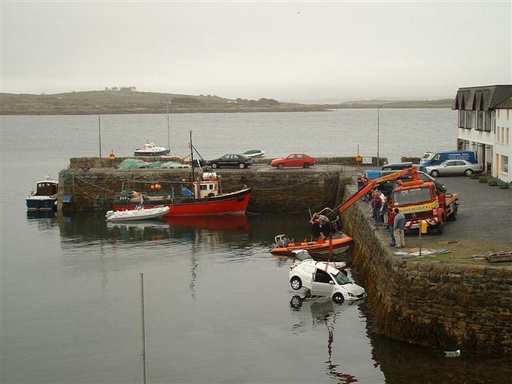
\includegraphics[width=\linewidth,height=.25\textheight,keepaspectratio]{images/image5.jpeg}
\end{minipage}\hfill
\begin{minipage}[c]{.48\linewidth}
\centering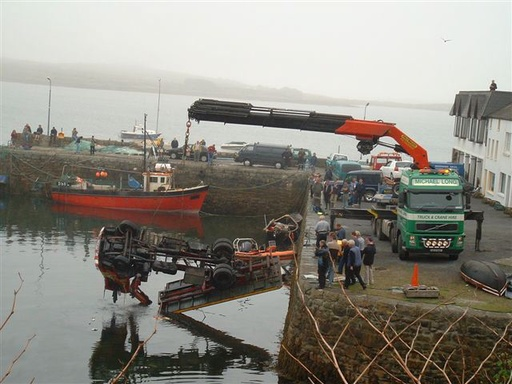
\includegraphics[width=\linewidth,height=.25\textheight,keepaspectratio]{images/image8.jpeg}
\end{minipage}
\end{center}

Les erreurs de conception apparaissent aussi lorsque les interfaces avec l'existant sont mal maîtrisées : gabarit d'un train et dimensions des quais, logiciel et réseau, véhicule et réglementation, produit et maintenance.

\section{Définir un système}\label{sec:is-systeme}

\begin{ISdefinition}
Un \textbf{système} est un ensemble d'éléments en interaction, organisé pour atteindre un ou plusieurs résultats quantifiables en termes de performance.
\end{ISdefinition}

Un système possède :
\begin{itemize}
  \item une finalité et des fonctions ;
  \item une frontière qui distingue le système de son environnement ;
  \item des constituants organisés selon une architecture ;
  \item des interfaces par lesquelles circulent matière, énergie et information ;
  \item des performances mesurables.
\end{itemize}

\ISSystemeBoiteNoire

\subsection{Systèmes naturels et artificiels}

Les systèmes naturels existent indépendamment d'une intention de conception : système solaire, organisme vivant ou écosystème. Les systèmes artificiels sont créés ou transformés par l'être humain pour répondre à un besoin.

En sciences industrielles, on étudie principalement des systèmes artificiels pluritechnologiques associant mécanique, électronique, informatique, automatique, énergie et communication.

\subsection{Frontière et environnement}

La frontière dépend de la question posée. Pour étudier l'autonomie d'un véhicule, la batterie appartient au système. Pour étudier la fabrication de cette batterie, les procédés industriels et les matières premières deviennent eux-mêmes des sous-systèmes étudiés.

\ISContexte

\begin{ISattention}
Une frontière mal définie conduit à oublier une interface ou à attribuer au système une performance qui dépend en réalité d'un élément extérieur. La frontière doit toujours être explicitée.
\end{ISattention}

\section{Besoin, fonction et solution}\label{sec:is-besoin}

\subsection{Besoin}

Le besoin décrit ce qu'attend une partie prenante sans imposer prématurément une solution technique. Il doit être formulé du point de vue du service rendu.

Exemple : « permettre à une personne à mobilité réduite de franchir un dénivelé en sécurité » est un besoin. « installer un moteur de 500 W » est déjà une solution.

\subsection{Fonctions de service et contraintes}

Une fonction de service exprime une action utile entre le système et son environnement. Une contrainte limite la liberté du concepteur : sécurité, norme, masse, encombrement, coût, environnement ou maintenance.

Une formulation efficace utilise un verbe à l'infinitif et un complément :
\begin{itemize}
  \item déplacer une charge ;
  \item informer l'utilisateur ;
  \item résister à l'humidité ;
  \item limiter les nuisances sonores.
\end{itemize}

\begin{ISmethode}[title={Formuler une exigence fonctionnelle}]
\begin{enumerate}
  \item Identifier la partie prenante concernée.
  \item Décrire le service attendu sans citer de solution.
  \item Associer un critère mesurable.
  \item Fixer un niveau et une flexibilité ou tolérance.
  \item Préciser le scénario de vérification.
\end{enumerate}
\end{ISmethode}

\section{Trois représentations du système}\label{sec:is-ecarts}

Au cours d'une démarche de conception, on distingue :
\begin{description}
  \item[Système souhaité :] défini par le besoin, les exigences et le cahier des charges ;
  \item[Système simulé :] représenté par des modèles numériques ou analytiques ;
  \item[Système réel :] prototype ou produit effectivement réalisé et mesuré.
\end{description}

\ISTriangleSystemes

Les trois écarts fondamentaux sont :
\begin{itemize}
  \item écart entre souhaité et simulé : qualité du modèle et choix de conception ;
  \item écart entre simulé et réel : incertitudes, hypothèses et réalisation ;
  \item écart entre réel et souhaité : conformité du produit au besoin.
\end{itemize}

La démarche expérimentale sert à quantifier ces écarts et à améliorer soit le produit, soit le modèle, soit la formulation des exigences.

\section{Cycle de vie d'un système}\label{sec:is-cycle-vie}

Le cycle de vie couvre l'ensemble des étapes depuis l'expression du besoin jusqu'au retrait de service :
\begin{enumerate}
  \item analyse du besoin et faisabilité ;
  \item spécification et conception ;
  \item réalisation et intégration ;
  \item vérification et validation ;
  \item production, exploitation et maintenance ;
  \item évolution, réemploi, recyclage ou élimination.
\end{enumerate}

La prise en compte du cycle de vie dès la conception évite de déplacer les problèmes vers la fabrication, l'utilisation, la maintenance ou la fin de vie.

\subsection{Approche environnementale}

L'analyse de cycle de vie évalue les consommations de ressources et les impacts environnementaux sur toutes les étapes. Elle évite qu'une amélioration locale ne crée un impact plus important ailleurs.

Les principales familles d'indicateurs concernent :
\begin{itemize}
  \item consommation d'énergie et de ressources non renouvelables ;
  \item émissions de gaz à effet de serre ;
  \item acidification, eutrophisation et toxicité ;
  \item déchets, bruit, occupation des sols et consommation d'eau.
\end{itemize}

\begin{ISapplication}[title={Éco-conception}]
Réduire la masse d'un produit peut diminuer l'énergie consommée pendant son usage, mais rendre le recyclage plus complexe si des matériaux composites indissociables sont utilisés. L'évaluation doit porter sur le cycle complet.
\end{ISapplication}
